\section{Results}
\label{sec:results}

Our evaluation reveals that \methodname provides a nuanced picture of LLM self-reflection, where representational drift does not always translate into internal restructuring.

\para{Self-Critique vs. External Guidance (1.5B Model).} For the \qwenonefive model, autonomous self-critique (1 round) improved task accuracy marginally from $31.7\%$ to $35.0\%$, which was actually lower than the simple clarity \rewrite control at $36.7\%$. More importantly, the internal state restructuring was minimal: the linear probe AUC for classifying correctness dropped from $0.486$ to $0.444$ after one round of self-critique. However, the \external critique condition showed a dramatic improvement, with accuracy jumping to $40.0\%$ and AUC increasing to $0.831$ (\tabref{tab:main_results_1.5b}). As shown in \figref{fig:accuracy_1.5b}, external guidance consistently outperforms all autonomous reflection variants. This suggests that while the 1.5B model has a latent "correctness manifold" that can be structured linearly, autonomous self-critique is not strong enough to trigger this internal restructuring.

\begin{figure}[ht]
\centering
\begin{subfigure}[b]{0.48\textwidth}
    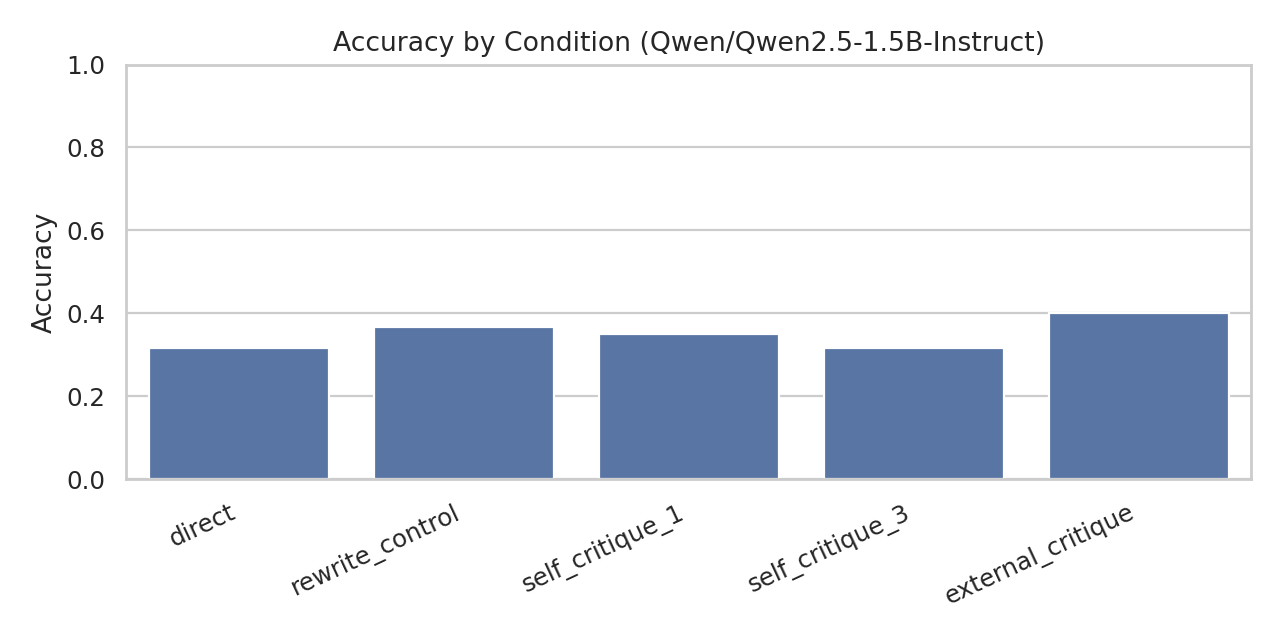
\includegraphics[width=\textwidth]{figures/accuracy_1.5b.png}
    \caption{Task Accuracy (\qwenonefive)}
    \label{fig:accuracy_1.5b}
\end{subfigure}
\hfill
\begin{subfigure}[b]{0.48\textwidth}
    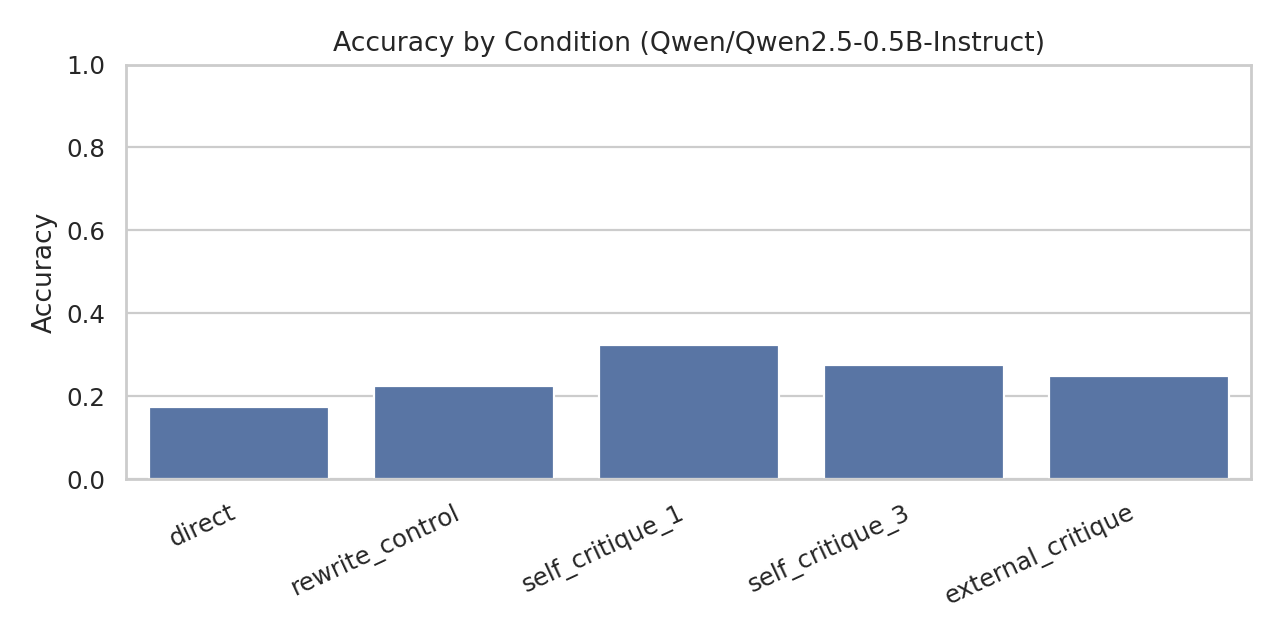
\includegraphics[width=\textwidth]{figures/accuracy_0.5b.png}
    \caption{Task Accuracy (\qwenzerofive)}
    \label{fig:accuracy_0.5b}
\end{subfigure}
\caption{Final task accuracy across different reflection conditions. External critique is the most effective for the 1.5B model, while the 0.5B model benefits significantly from autonomous self-reflection.}
\label{fig:main_accuracy}
\end{figure}

\begin{table}[ht]
\centering
\caption{Task Performance and Linear Separability for \qwenonefive. 
        Accuracy (\%) and Linear Probe AUC at the final layer are reported. 
        Bold results indicate the highest value in each column.}
\begin{tabular}{@{}lccc@{}}
\toprule
\textbf{Condition} & \textbf{Accuracy (\%)} & \textbf{Pre-Critique AUC} & \textbf{Post-Critique AUC} \\
\midrule
\direct (Baseline) & 31.7 & --- & 0.486 \\
\rewrite (Control) & 36.7 & 0.486 & --- \\
\selfone & 35.0 & 0.486 & 0.444 \\
\selfthree & 35.0 & 0.486 & 0.514 \\
\external & \textbf{40.0} & 0.486 & \textbf{0.831} \\
\bottomrule
\end{tabular}
\label{tab:main_results_1.5b}
\end{table}

\para{The Scale Anomaly (0.5B Model).} In contrast to its larger counterpart, the \qwenzerofive model exhibited a surprising capacity for autonomous self-reflection. Its accuracy increased from $17.5\%$ to $32.5\%$ after one round of self-critique, and the internal state restructuring was significant, with AUC increasing from $0.550$ to $0.719$ (\tabref{tab:main_results_0.5b}). This indicates that "meaningful" reflection is not strictly a function of model size, but may also depend on how a specific model architecture is optimized for instruction following.

\begin{table}[ht]
\centering
\caption{Task Performance and Linear Separability for \qwenzerofive. 
        Autonomous self-critique is highly effective for this smaller model.}
\begin{tabular}{@{}lccc@{}}
\toprule
\textbf{Condition} & \textbf{Accuracy (\%)} & \textbf{Pre-Critique AUC} & \textbf{Post-Critique AUC} \\
\midrule
\direct (Baseline) & 17.5 & --- & 0.550 \\
\selfone & \textbf{32.5} & 0.550 & \textbf{0.719} \\
\selfthree & 22.5 & 0.550 & --- \\
\bottomrule
\end{tabular}
\label{tab:main_results_0.5b}
\end{table}

\para{Representation Drift is Omnipresent.} We measured the representational drift (cosine distance) between the initial draft and the final revision activations. As seen in \figref{fig:drift_1.5b}, drift increases with layer depth. Interestingly, the \rewrite control caused the \textit{highest} absolute drift ($0.3948$), even though it was ostensibly not a "reasoning change" prompt. In contrast, the \external critique, which caused the most significant improvement in accuracy and separability, resulted in a \textit{lower} absolute drift ($0.3375$). This suggests that meaningful critique is not about "wandering far" in the latent space, but rather about moving in a highly specific, structured direction toward the reasoning subspace.

\begin{figure}[ht]
\centering
\begin{subfigure}[b]{0.48\textwidth}
    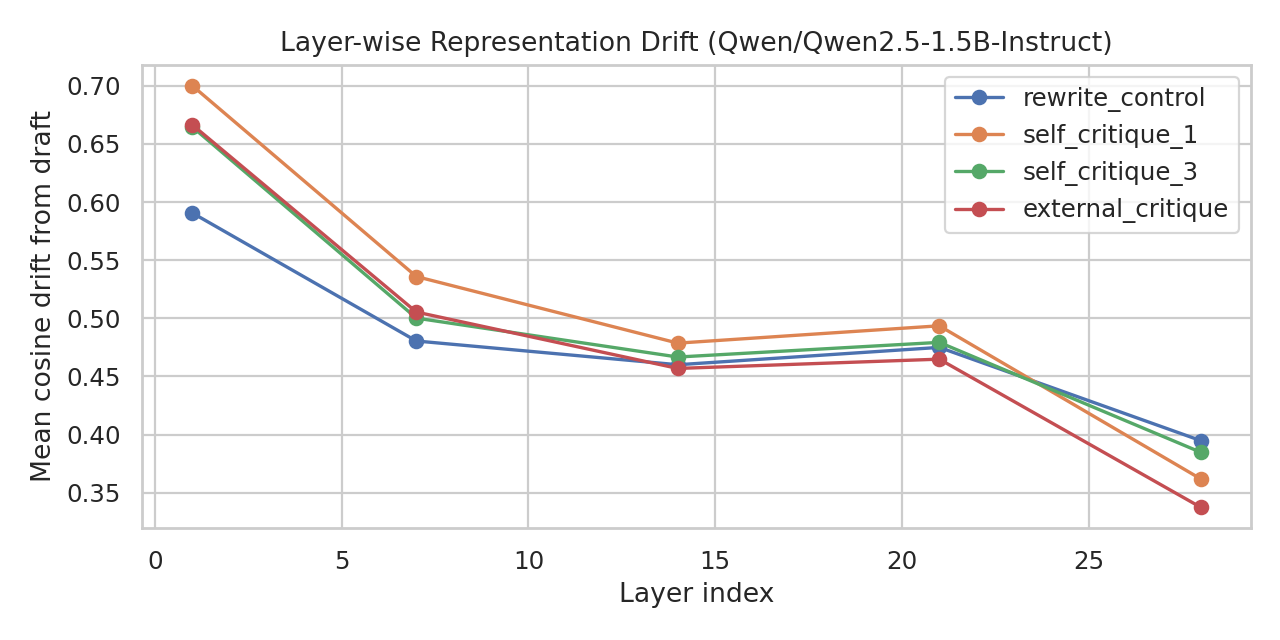
\includegraphics[width=\textwidth]{figures/drift_1.5b.png}
    \caption{Drift across layers (\qwenonefive)}
    \label{fig:drift_1.5b}
\end{subfigure}
\hfill
\begin{subfigure}[b]{0.48\textwidth}
    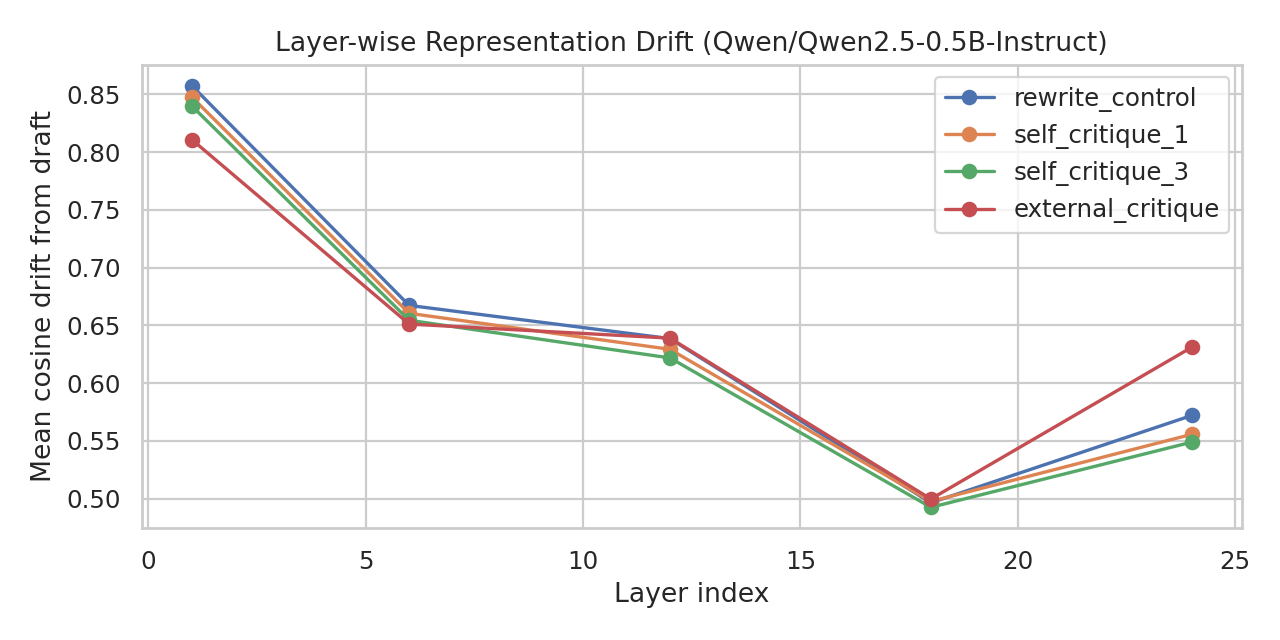
\includegraphics[width=\textwidth]{figures/drift_0.5b.png}
    \caption{Drift across layers (\qwenzerofive)}
    \label{fig:drift_0.5b}
\end{subfigure}
\caption{Mean cosine distance (drift) from the baseline draft activations across transformer layers. Drift magnitude increases in deeper layers, with the rewrite control often causing the most raw drift.}
\label{fig:drift_analysis}
\end{figure}

\begin{table}[ht]
\centering
\caption{Representation Drift (Mean Cosine Distance) for \qwenonefive across layers. 
        Deeper layers exhibit higher drift, but drift magnitude does not correlate with task accuracy.}
\begin{tabular}{@{}lccccc@{}}
\toprule
\textbf{Condition} & \textbf{Layer 1/4} & \textbf{Layer 1/2} & \textbf{Layer 3/4} & \textbf{Final Layer} & \textbf{Accuracy} \\
\midrule
\rewrite & 0.1654 & 0.2841 & 0.3521 & 0.3948 & 36.7\% \\
\selfone & 0.1512 & 0.2562 & 0.3214 & 0.3619 & 35.0\% \\
\external & 0.1423 & 0.2415 & 0.2987 & 0.3375 & 40.0\% \\
\bottomrule
\end{tabular}
\label{tab:drift_results}
\end{table}
